% Gerado por scripts/gerar-figuras-monografia.py; não editar.
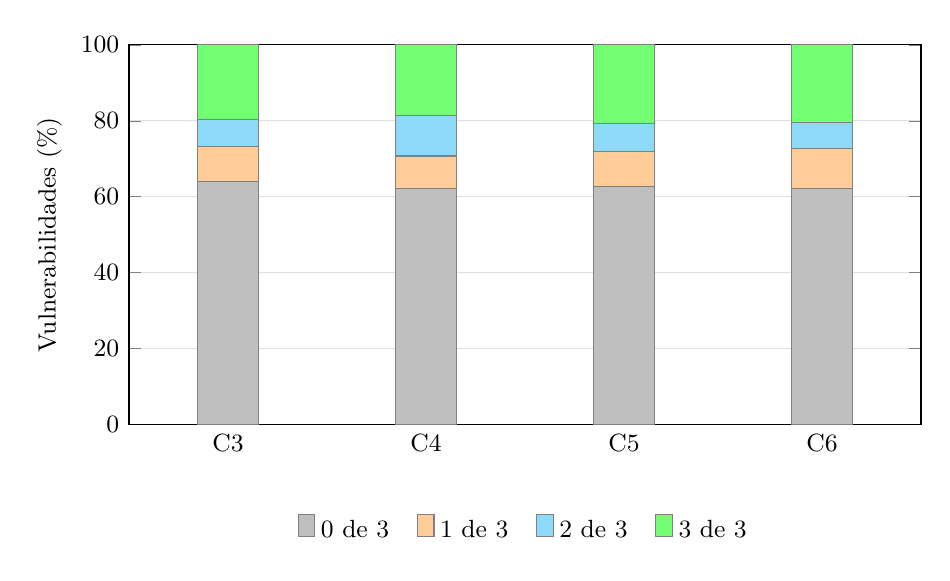
\begin{tikzpicture}
\begin{axis}[
width=0.96\textwidth,height=6.4cm,
tick label style={font=\small},label style={font=\small},
legend style={font=\small,at={(0.5,-0.22)},anchor=north,legend columns=3,draw=none,/tikz/every even column/.append style={column sep=8pt}},
ymajorgrids=true,grid style={black!12},
ybar stacked,bar width=22pt,xmin=0.5,xmax=4.5,ymin=0,ymax=100,ylabel={Vulnerabilidades (\%)},xtick={1,2,3,4},xticklabels={C3,C4,C5,C6},legend columns=4
]
\addplot+[fill=black!25,draw=black!50] coordinates {(1,63.98852224) (2,62.12338594) (3,62.69727403) (4,62.12338594)};
\addlegendentry{0 de 3}
\addplot+[fill=orange!40,draw=black!50] coordinates {(1,9.32568149) (2,8.60832138) (3,9.18220947) (4,10.61692970)};
\addlegendentry{1 de 3}
\addplot+[fill=cyan!45,draw=black!50] coordinates {(1,7.03012912) (2,10.61692970) (3,7.46054519) (4,6.88665710)};
\addlegendentry{2 de 3}
\addplot+[fill=green!55,draw=black!50] coordinates {(1,19.65566714) (2,18.65136298) (3,20.65997131) (4,20.37302726)};
\addlegendentry{3 de 3}
\end{axis}
\end{tikzpicture}
